\documentclass{article}

\usepackage[a4paper,top=3cm,bottom=2cm,left=3cm,right=3cm,marginparwidth=1.75cm]{geometry}
\usepackage[english]{babel}
\usepackage[utf8]{inputenc}
\usepackage{amsmath}
\usepackage{amsfonts}
\usepackage{graphicx}
\usepackage{url}
\usepackage[colorlinks=true, allcolors=blue]{hyperref}

\title{Project: flows on 3D surfaces}
\author{Daw Lara, Pignotti Simone, Revuz Anselme}

\begin{document}
\maketitle

\section*{Introduction}
The goal of the project was to implement different kind of flows for 3D surfaces
using the programming framework Processing, and to compare the results obtained
on multiple surfaces given as PLY files. We have implemented ...

\section*{Documentation}
To implement the interface, we used the Processing library G4P. To install it,
open the IDE of Processing (tested on v3.3.6), got to the ``Sketch'' menu, click on
``Import Library...'', and finally ``Add Library...''. In the window which appears,
search "g4p" in the field ``Filter'' and install ``G4P'' (tested on v4.1.4 of such library).\\

The main menu is composed by three elements:
\begin{itemize}
  \item the ``NEW'' button, allowing to open a new window;
  \item the ``Start/Stop flow'' button, allowing to start or stop the flow on every window;
  \item a list of clickable buttons for opening each window's parameter menu.
\end{itemize}

\begin{center}

\end{center}
\begin{figure}[h]
  \begin{center}
    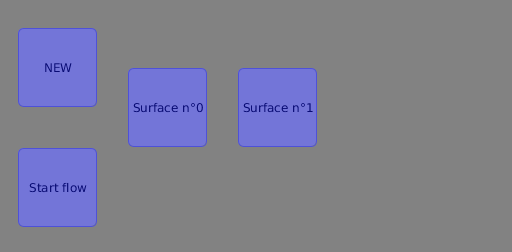
\includegraphics[width=.5\textwidth]{img/main.png}
    \caption{Main menu}
    \label{fig:main}
  \end{center}
\end{figure}

When clicking on the button associated to a window, a new menu appears
allowing to modify the following parameters:
\begin{itemize}
  \item the flow to apply, encoded by an integer, namely:
  \begin{enumerate}
    \item mean curvature with volume renormalization;
    \item mean curvature with projection on the volume constraints;
    \item harmonic with volume renormalization;
    \item harmonic with projection on the volume constraints;
    \item harmonic with division by the area and volume renormalization;
    \item harmonic with division by the area and projection on the volume constraints;
    \item squared mean curvature with volume renormalization;
    \item squared mean curvature with projection on the volume constraints;
  \end{enumerate}
  \item the value of ``tau'', a float $0 \leq \tau \leq 1$ representing the scaling factor applied to the flow;
  \item the PLY file to use, with examples provided in the data directory;
  \item the activity of the flow on the current window,
    allowing to stop the flow on it even if start flow was pressed in the main menu.
\end{itemize}

\begin{figure}[h]
  \begin{center}
    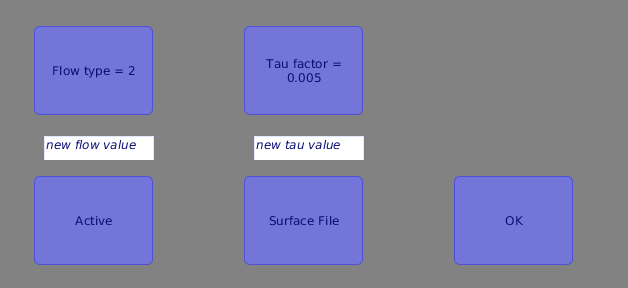
\includegraphics[width=.5\textwidth]{img/win_params.png}
    \caption{Parameters of each window}
    \label{fig:win_params}
  \end{center}
\end{figure}

At creation, a window opens the cube surface, with no flow applied and $\tau = 0.005$.
Once created, the windows cannot be closed. To disable the flow on a window,
choose a negative integer.

The value of $\tau$ is parsed as a float, so it is expected to be a floating point
number in the standard notation.

The button ``OK'' allows to go back to the main menu, but every modification
is immediately applied, even without pressing ``OK''.

When a window is selected, the keys 'A' and 'Z' allows to zoom in and out, respectively.

\begin{figure}[h]
  \begin{center}
    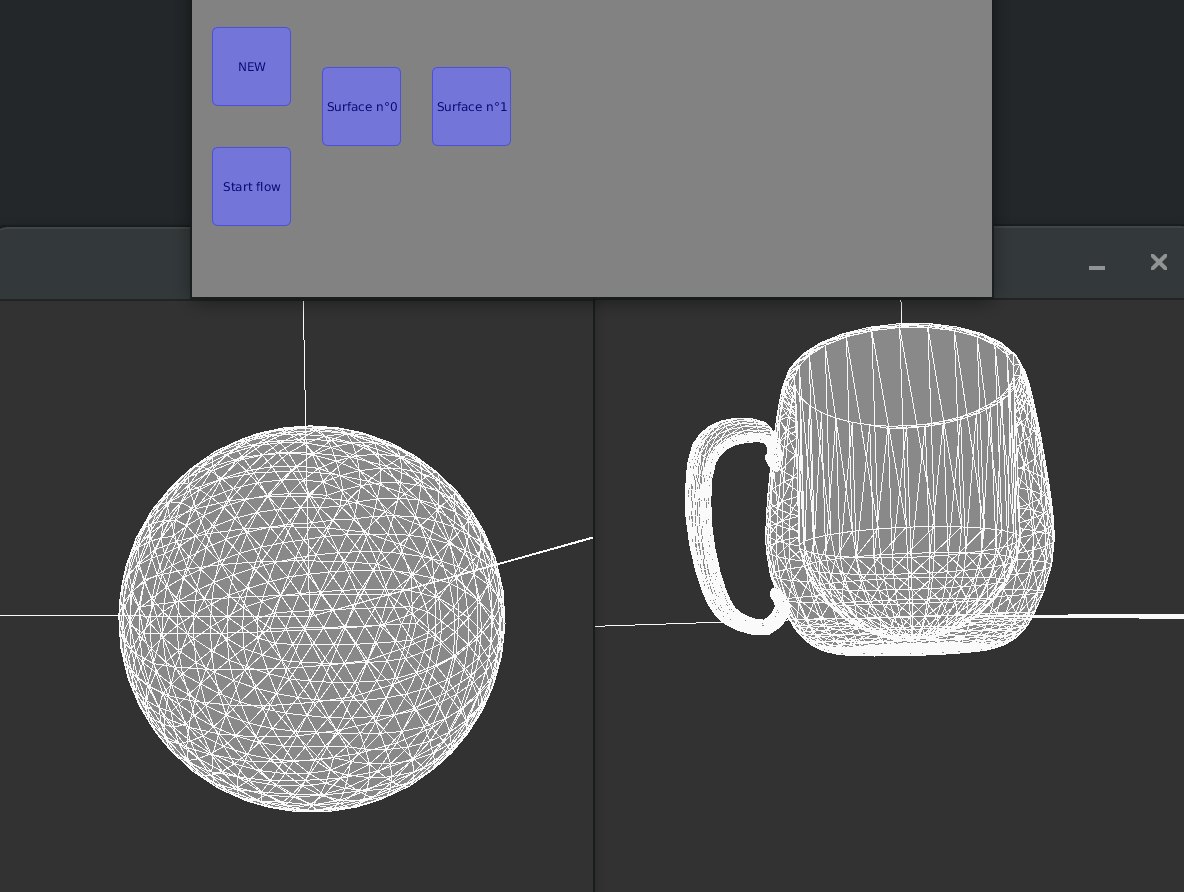
\includegraphics[width=.5\textwidth]{img/mult.png}
    \caption{Multiple windows synchronously applying different flows on different surfaces}
    \label{fig:mult}
  \end{center}
\end{figure}

\section*{Implementation of the flows}

\paragraph*{HarmonicFlow:}
For each vertex $p_i$, compute the set of adjacent vertices $N_i$.
For each $p_j \in N_i$, add $p_j$ to $\overrightarrow{H_i}$, and divide by
the cardinality of $N_i$.
\begin{equation*}
  \overrightarrow{H_i}=\frac{1}{|N_i|} \sum_{p_j \in N_i} \overrightarrow{p_j}
\end{equation*}
\paragraph*{HarmonicAreaFlow:}
For each vertex $p_i$, compute the set of adjacent vertices $N_i$.
First, calculate the harmonic flow $\overrightarrow{H_i}$ as above, then divided by the area
calculated in the following way:
\begin{equation*}
  A_i = \frac{1}{2} \sum_{j = 1}^{|N_i|} (\overrightarrow{N_i[j] P_i} \times \overrightarrow{N_i[j+1] N_i[j]} )
\end{equation*}
Finally the flow will yield:
\begin{equation*}
  \overrightarrow{H_i}=\frac{1}{A_i} \left( \frac{1}{|N_i|} \sum_{p_j \in N_i} \overrightarrow{p_j} \right)
\end{equation*}
\paragraph*{MeanCurvatureFlow:}
For each vertex,
We used the following notations :
Q is the point we calculate the mcf for in each iteration
$P_i$ is the predecessor of Q on face j, the successor of Q on face (j+1) and therefore the shared vertex of faces (j, j+1)
$P_{i-1}$ is the successor of Q on face j
$P_{i+i}$ is the predecessor of Q on face (j+1)
$\overrightarrow{M_i}$ is the edge ($P_i$, Q)
We applied the following steps:
- We find the first incident face f and the predecessor and the successor of Q in f
- We iterate over the face in the right order by finding  the face show contain Q and its predecessor
- The flow will be:
\begin{center}
$mcf[i]=\frac{-1}{2}\sum_{f}^{} \frac{\overrightarrow{QP_{i-1}} *\overrightarrow{QP_{i-1}}}{||\overrightarrow{QP_{i-1}} *\overrightarrow{QP_{i-1}}||} * \overrightarrow{P_iP_{i-1}} $
\end{center}
\paragraph*{MeanCurvatureFlowCotan:}
For each vertex,
We used the following notations :
Q is the point we calculate the mcf for in each iteration
$P_i$ is the predecessor of Q on face j, the successor of Q on face (j+1) and therefore the shared vertex of faces (j, j+1)
$P_{i-1}$ is the successor of Q on face j
$P_{i+i}$ is the predecessor of Q on face (j+1)
$\overrightarrow{M_i}$ is the edge ($P_i$, Q)
$angelbefore = (\overrightarrow{QP_{i-1}},\overrightarrow{P_{i-1}P_{i}})$
$angelafter = (\overrightarrow{P_iP_{i+1}},\overrightarrow{P_{i+1}Q})$
We applied the following steps:
- We find the first incident face f and the predecessor and the successor of Q in f
- We iterate over the face in the right order by finding  the face show contain Q and its predecessor
- The flow will be:
\begin{center}
$mcf[i]= \frac{1}{2}\sum_{f}^{} (\frac{1}{\tan angelbefore}+ \frac{1}{\tan after} ) * M_i$
\end{center}
\paragraph*{VolumeConservationFlow:}
\textit{Step 1:} (Gradient)
For each vertex $P_i$, we loop over the faces and for the incident face we do the following steps:
- Find the position of $P_i$ in this face
-We loop over all the vertices other than $P_i$ two by two and calculate their cross product :\\ $detP= \overrightarrow{P_1} * \overrightarrow{P_2} $
The gradient will be array of all these detP.
\textit{Step 2:} (Renormalization of the flow)
For each vertex $P_i$, the flow will be :
\begin{center}
$\overrightarrow{F}= \overrightarrow{H}- \frac{\overrightarrow{detP}. \overrightarrow{H}}{\overrightarrow{detP}. \overrightarrow{detP}}\overrightarrow{detP}$
\end{center}

\end{document}
